\documentclass[preprint,12pt]{elsarticle}

\usepackage{ctex}
\usepackage{amssymb}
\usepackage{amsmath}
\usepackage{graphicx}
\usepackage{booktabs}
\usepackage{geometry}
\usepackage{hyperref}
\usepackage{subcaption}
\usepackage{caption}
\usepackage{float}
\usepackage{algorithm}
\usepackage{algpseudocode}
\usepackage{multirow}
\usepackage{array}
\usepackage{enumitem}

\graphicspath{{./figures/}}
\journal{Journal of Manufacturing Systems}

\renewcommand{\algorithmicrequire}{\textbf{Require:}}
\renewcommand{\algorithmicensure}{\textbf{Ensure:}}

\begin{document}

\begin{frontmatter}

\title{基于前瞻距离与捷度约束的数控机床强化学习运动规划方法}

\author[1]{作者姓名}
\affiliation[1]{organization={某某大学/机构},
            addressline={某某路},
            city={某某市},
            postcode={000000},
            country={中国}}

\begin{abstract}
针对传统数控刀具规划的路径，从轨迹平滑到速度规划的传统流程在拐角处难以同时兼顾效率、平滑性与运动学约束。本文提出一种考虑捷度约束的端到端强化学习运动规划框架，将路径跟踪建模为允差带内的受约束序列决策问题。本文目标为在同一决策闭环内同时处理拐角平滑、速度规划和运动学约束问题，避免轨迹平滑与速度规划割裂，同时输出满足运动学约束的插补序列。状态由核心运动学量、拐角感知量和多尺度前瞻几何量组成，策略动作包含转向分量、进给分量和前瞻距离调节分量；执行阶段引入运动学约束模块，对转向与进给分量映射得到的约束前运动控制量进行在线约束投影，使插补序列的速度、加速度与捷度满足约束。设计了圆形、正方形、蝴蝶形三条代表性路径作为实验路径，实验证明，在该框架下，策略能够在允差带内灵活选择路径来得到更平滑的规划轨迹，同时满足速度、加速度与捷度约束，提升了复杂路径下运动规划结果的动态可执行性与拐角通过平滑性。
\end{abstract}

\begin{keyword}
运动规划 \sep 强化学习 \sep 捷度约束 \sep 端到端控制 \sep CNC
\end{keyword}

\end{frontmatter}

\section{引言}
\label{sec:intro}

现代高端数控（CNC）加工中，复杂自由曲面的刀具路径通常仍以长直线、短直线与圆弧混合的形式输入到控制系统。对于这类混合路径，运动规划决定加工效率，直接影响轮廓精度、表面质量与伺服运行平稳性。Sun 等\cite{Sun2022}的综述将自由曲面加工的关键问题概括为刀具路径生成、进给率规划与轨迹规划三个层面，并指出这三者在实际插补执行中通过离散程序段之间的局部过渡紧密关联。当长短线段密集交接、直线与圆弧频繁切换或局部曲率快速变化时，若几何处理与动态约束协调不足，会引起进给骤降、轮廓误差超限以及机床振动等问题。已有研究表明，这一现象在 NURBS 自适应平滑插补\cite{Xu2022}、五轴时间样条插补\cite{Wu2023}以及五轴 B 样条平滑\cite{Hu2024}等场景中均有出现。针对“长短直线与圆弧交加”这一典型工况，Li 等\cite{Li2023}进一步指出，几何过渡设计与速度规划之间的耦合不足会直接限制加工效率与表面质量。

围绕上述问题，现有 CNC 运动规划通常可分为几何层轨迹平滑与时间层速度规划两个相互衔接的环节。Yan 等\cite{Yan2023}在其拐角平滑综述中指出，几何层的研究目标是对离散程序段之间的连接关系进行重构，以减小拐角处的几何不连续并改善后续运动的可执行性。其中一类方法属于局部拐角平滑，在相邻程序段之间插入圆弧、Bezier 曲线或 B 样条过渡段以控制拐角误差并提升高阶导数连续性。Zhao 等\cite{Zhao2013}提出了基于曲率连续 B 样条过渡的实时前瞻插补方法，Fan 等\cite{Fan2015}进一步给出了短线段加工中的曲率平滑插补与运动规划方案。在尖角处理方面，Sencer 等\cite{Sencer2015}提出了面向高速进给的曲率最优尖角平滑算法，Tajima 与 Sencer\cite{Tajima2016}从运动学角度对拐角平滑进行了系统设计，Li 等\cite{Li2023}则针对直线与圆弧混合刀具路径提出了基于运动重叠策略的集成平滑方法。另一类方法属于全局平滑或全局拟合，通过对连续短线段进行整体重构或统一优化来改善密集短线段场景下的整体连续性。Tajima 与 Sencer\cite{Tajima2017,Tajima2022}先后给出了无中断加速的全局刀具路径平滑方法以及面向五轴加工的在线插补全局混合方案；Song 等\cite{Song2021}采用控制点分配结合 FIR 滤波运动平滑实现短线段刀具路径的全局平滑；Sun 等\cite{Sun2024}进一步针对五轴刀具路径提出了进给波动更小、计算效率更高的平滑插补方法。在时间层，研究重点是在给定几何路径或平滑轨迹的基础上进行速度规划，在弦高误差、伺服驱动能力、加速度与捷度等约束下对速度曲线进行规划。Erkorkmaz 与 Altintas\cite{Erkorkmaz2001}较早建立了捷度受限的轨迹生成与五次样条插补框架。在 NURBS 等参数化路径上，Lee 等\cite{Lee2011}提出了 NURBS 插补的进给率调度方法，Wu 等\cite{Wu2022}给出了驱动与弦误差约束下结合三次与四次 S 型曲线的 NURBS 进给率调度方案。在轴约束与高阶约束方面，Song 等\cite{Song2020}面向五轴长样条刀具路径提出了基于轴驱动约束的前瞻窗口区间自适应进给率调度方法，Zhang 等\cite{Zhang2021}则在参数化刀具路径上引入了法向捷度约束的自适应进给率规划与迭代插补器。近期，Zhang 等\cite{Zhang2026}通过约束引导采样实现捷度受限的进给率调度，Wang 等\cite{Wang2025b}则进一步面向非平稳边界条件给出了捷度受限的无振荡进给率调度方案。上述方法为高速高精加工提供了重要基础，但其适用边界也较为明确：局部平滑方法通常受限于段长和邻域重叠关系\cite{Zhao2013,Tajima2016,Li2023}；全局方法虽然更适合处理密集短线段，但需要在原始路径特征保持、实时性与实现复杂度之间进行权衡\cite{Tajima2017,Song2021}。在多数串行框架中，几何层处理与时间层规划仍然相对分离，使空间几何参数与时间标定参数之间只能间接协调，在混合路径下容易出现保守降速、前后段速度衔接不稳或局部动态性能利用不足等问题\cite{Yan2023,Wang2025}。

近年来，学习方法为复杂路径运动控制提供了不同于规则驱动模型的另一条技术路线。在更广泛的制造优化场景中，深度表征学习与强化学习已被用于 CNC 相关决策问题，表明学习方法在加工智能化中的应用基础正在形成 \cite{Samsonov2023}。在运动规划方向，Li 等 \cite{Li2020} 提出了一种基于强化学习训练的神经网络直接轨迹平滑方法，按插补周期直接输出伺服指令，实现了复杂刀具路径下的轨迹平滑与连续运动控制。这类工作说明，强化学习可以进入 CNC 轨迹平滑控制环节，并从路径特征与运行状态中直接学习控制行为 \cite{Li2020}。但需要指出的是，该类研究的重点在于学习型轨迹平滑控制本身，而不是将其明确构造成轨迹平滑与速度规划协同优化的统一框架。在此基础上，近期相关研究进一步开始强调几何、动力学与感知信息的协同设计。一方面，关于路径规划与轨迹平滑一致性的讨论正在增多。Wang 等\cite{Wang2025}从曲面评估视角研究了 CNC 加工中路径平滑与轨迹规划的一致性，强调了几何过渡质量与后续速度规划之间的耦合关系；Zhang 等\cite{Zhang2026}与 Wang 等\cite{Wang2025b}则分别针对严格捷度约束与非平稳边界条件下的进给率调度问题给出了新的解决方案。另一方面，也有工作尝试将强化学习与轨迹生成模块结合：Alizadeh Kolagar 等\cite{Alizadeh2024}将深度强化学习与捷度有界轨迹生成器结合，以提高学习策略在运动学约束下的可执行性；面向轨迹平滑与进给率规划协同优化的学习型框架也开始出现\cite{KIRL2025}。此外，动态前瞻范围与多维状态反馈对于提前感知局部几何变化、减少不必要降速以及改善全局速度协调同样重要，Zhong 等\cite{Zhong2025}基于视觉反馈给出了工业机器人的实时动态前瞻轨迹规划方法。在相邻研究中，围绕混合机器人、五轴加工和机器人铣削等对象，已有工作分别从同步运动\cite{Zhang2024b}、姿态平滑\cite{Liu2024}以及刚度与平滑性协同优化\cite{Chen2024}等角度开展研究，主动—被动混合进给率控制也被用于抑制力波动并延长刀具寿命\cite{Li2024}，这些研究共同表明单纯依赖几何层或速度层的局部修补已难以覆盖复杂运动场景的需求。尽管如此，面向实际加工中“长短直线与圆弧交加”的混合刀具路径，现有方法仍存在三方面不足。其一，传统串行式框架下几何平滑与速度规划相互分离\cite{Sun2022,Yan2023}，难以在同一闭环内协调轮廓误差、过弯效率与运动学约束；其二，前瞻范围多由固定规则给定，难以随直线巡航、拐角临近和过弯阶段的变化在线调节；其三，即便引入学习策略，若缺少执行层的显式运动学约束，策略输出仍可能与速度、加速度和捷度边界不一致\cite{Li2020,Alizadeh2024,KIRL2025}。

为解决上述问题，本文提出了一种基于前瞻距离与捷度约束的数控机床强化学习运动规划方法。该方法在状态空间中联合核心运动学量、拐角特征与多尺度前瞻几何信息，在动作空间中设置前瞻距离调节分量，使其与转向分量、进给分量共同由策略输出；同时，设计运动学约束模块（Kinematic Constraint Module, KCM），对策略输出中的转向与进给分量映射得到的约束前运动控制量进行在线约束修正，使执行控制量满足速度、加速度与捷度限制；在奖励设计上，引导策略在同一决策闭环内协调轨迹偏移、路径进给与运动平滑性。传统串行式运动规划框架与本文运动规划框架在信息流、约束处理位置以及前瞻调节方式上的差异如图~\ref{fig:comparison_arch}所示。

\begin{figure}[htbp]
    \centering
    
\includegraphics[width=0.9\linewidth]{fig1.pdf}
    \caption{传统串行式运动规划与本文运动规划框架对比。}
    \label{fig:comparison_arch}
\end{figure}

本文的主要贡献如下：
\begin{enumerate}[leftmargin=2em]
    \item 构建了一种面向混合路径运动规划的状态表示，将实时运动学状态、拐角感知信息与多尺度前瞻几何信息统一到同一决策输入中；
    \item 将前瞻距离纳入动作空间，使策略能够根据直线进给、拐角临近和过弯阶段的差异在线调整感知尺度；
    \item 设计了嵌入强化学习闭环的运动学约束模块，通过在线约束修正将策略输出中的运动控制分量转换为满足速度、加速度与捷度限制的执行控制量；
\end{enumerate}

本文余下内容安排如下：第二章给出问题定义与约束建模；第三章介绍所提出的方法；第四章给出实验设置、评价指标与结果分析；第五章给出局限性分析与未来展望。

\section{问题定义与约束建模}
\label{sec:problem}

本章给出与本文方法直接相关的任务定义、几何约束与执行约束，为后续方法部分提供必要的形式化基础。

\subsection{刀具路径与几何可行域}
给定由CAM系统生成的离散刀位点序列
\begin{equation}
P_{raw}=\{p_1,p_2,\dots,p_N\},
\end{equation}
其中 $p_i\in\mathbb{R}^2$ 表示插补平面内的参考点。设轮廓允差为 $\varepsilon$，则参考路径两侧各偏置 $\varepsilon/2$ 后可得到一条允许策略局部偏离的几何可行域：
\begin{equation}
\Omega=\{x\mid d(x,P_{raw})\leq \varepsilon/2\},
\label{eq:feasible_region}
\end{equation}
式中 $d(x,P_{raw})$ 为点 $x$ 到参考路径的最小距离。该定义意味着允许策略在允差带内进行局部几何重分配，以换取更平滑的拐角通过过程,不是严格贴近原始轨迹。

\begin{figure}[htbp]
    \centering
    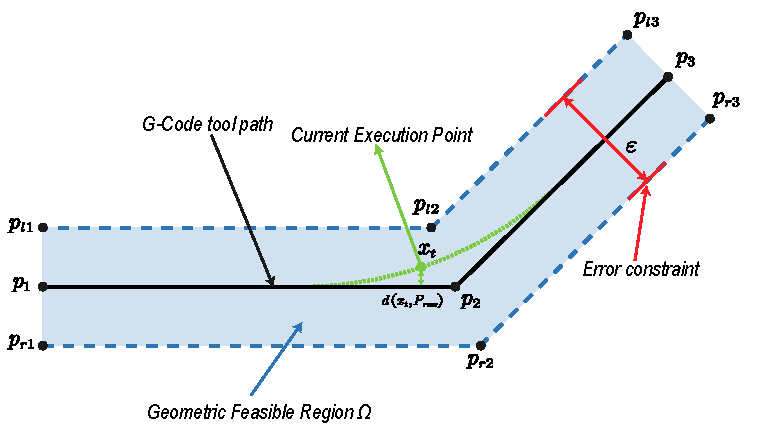
\includegraphics[width=0.9\linewidth]{fig2.pdf}
    \caption{参考路径与轮廓允差带构成的几何可行域。}
    \label{fig:feasible_region}
\end{figure}

为便于在闭环决策中感知局部几何，我们进一步对参考路径进行弧长参数化，并在当前投影弧长 $\ell_t$ 附近提取法向误差、切向方向、到下一拐角距离以及下一拐角转角等量。这些量既参与状态构造，也参与奖励加权与拐角模式判定。

\subsection{受约束动作决策表述}
在每个插补周期 $\Delta t$ 内，策略接收当前状态 $s_t$ 并输出归一化动作 $a_t^{\pi}$。KCM 输出的执行控制量作用于环境后，环境更新位置、姿态及运动学状态，并返回即时奖励 $r_t$。因此，本文任务可以写成一个受约束的序列决策问题：
\begin{equation}
\max_{\pi}\ \mathbb{E}_{\pi}\left[\sum_{t=0}^{T} \gamma^t r_t\right],
\end{equation}
同时满足几何约束
\begin{equation}
x_t\in \Omega,
\end{equation}
以及执行侧运动学约束
\begin{equation}
|v_t|\leq V_{\max},\quad |a_t|\leq A_{\max},\quad |j_t|\leq J_{\max},
\end{equation}
\begin{equation}
|\omega_t|\leq \Omega_{\max},\quad |\dot{\omega}_t|\leq A^{\omega}_{\max},\quad |\ddot{\omega}_t|\leq J^{\omega}_{\max}.
\end{equation}
其中 $v_t,a_t,j_t$ 分别表示线速度、线加速度与线捷度，$\omega_t,\dot{\omega}_t,\ddot{\omega}_t$ 分别表示角速度、角加速度与角捷度。

\section{方法}
\label{sec:method}

\subsection{总体框架}
本文方法的总体框架如图\ref{fig:framework}所示。给定参考路径与轮廓允差，系统首先在环境侧完成路径投影、拐角扫描与前瞻几何提取，构造当前时刻的结构化状态向量；随后，策略网络输出归一化动作，其中转向分量与进给分量被映射为约束前运动控制量 $(\omega_t^{pre},v_t^{pre})$，前瞻分量被映射为当前前瞻距离 $L_t$；最后，KCM 根据上一时刻的速度、加速度和捷度状态，对 $(\omega_t^{pre},v_t^{pre})$ 进行在线约束投影，得到满足速度、加速度与捷度限制的执行控制量 $(\omega_t,v_t)$。执行结果反过来更新当前位置、运动学量、拐角相位与前瞻观测，形成完整闭环。

\begin{figure}[htbp]
    \centering
    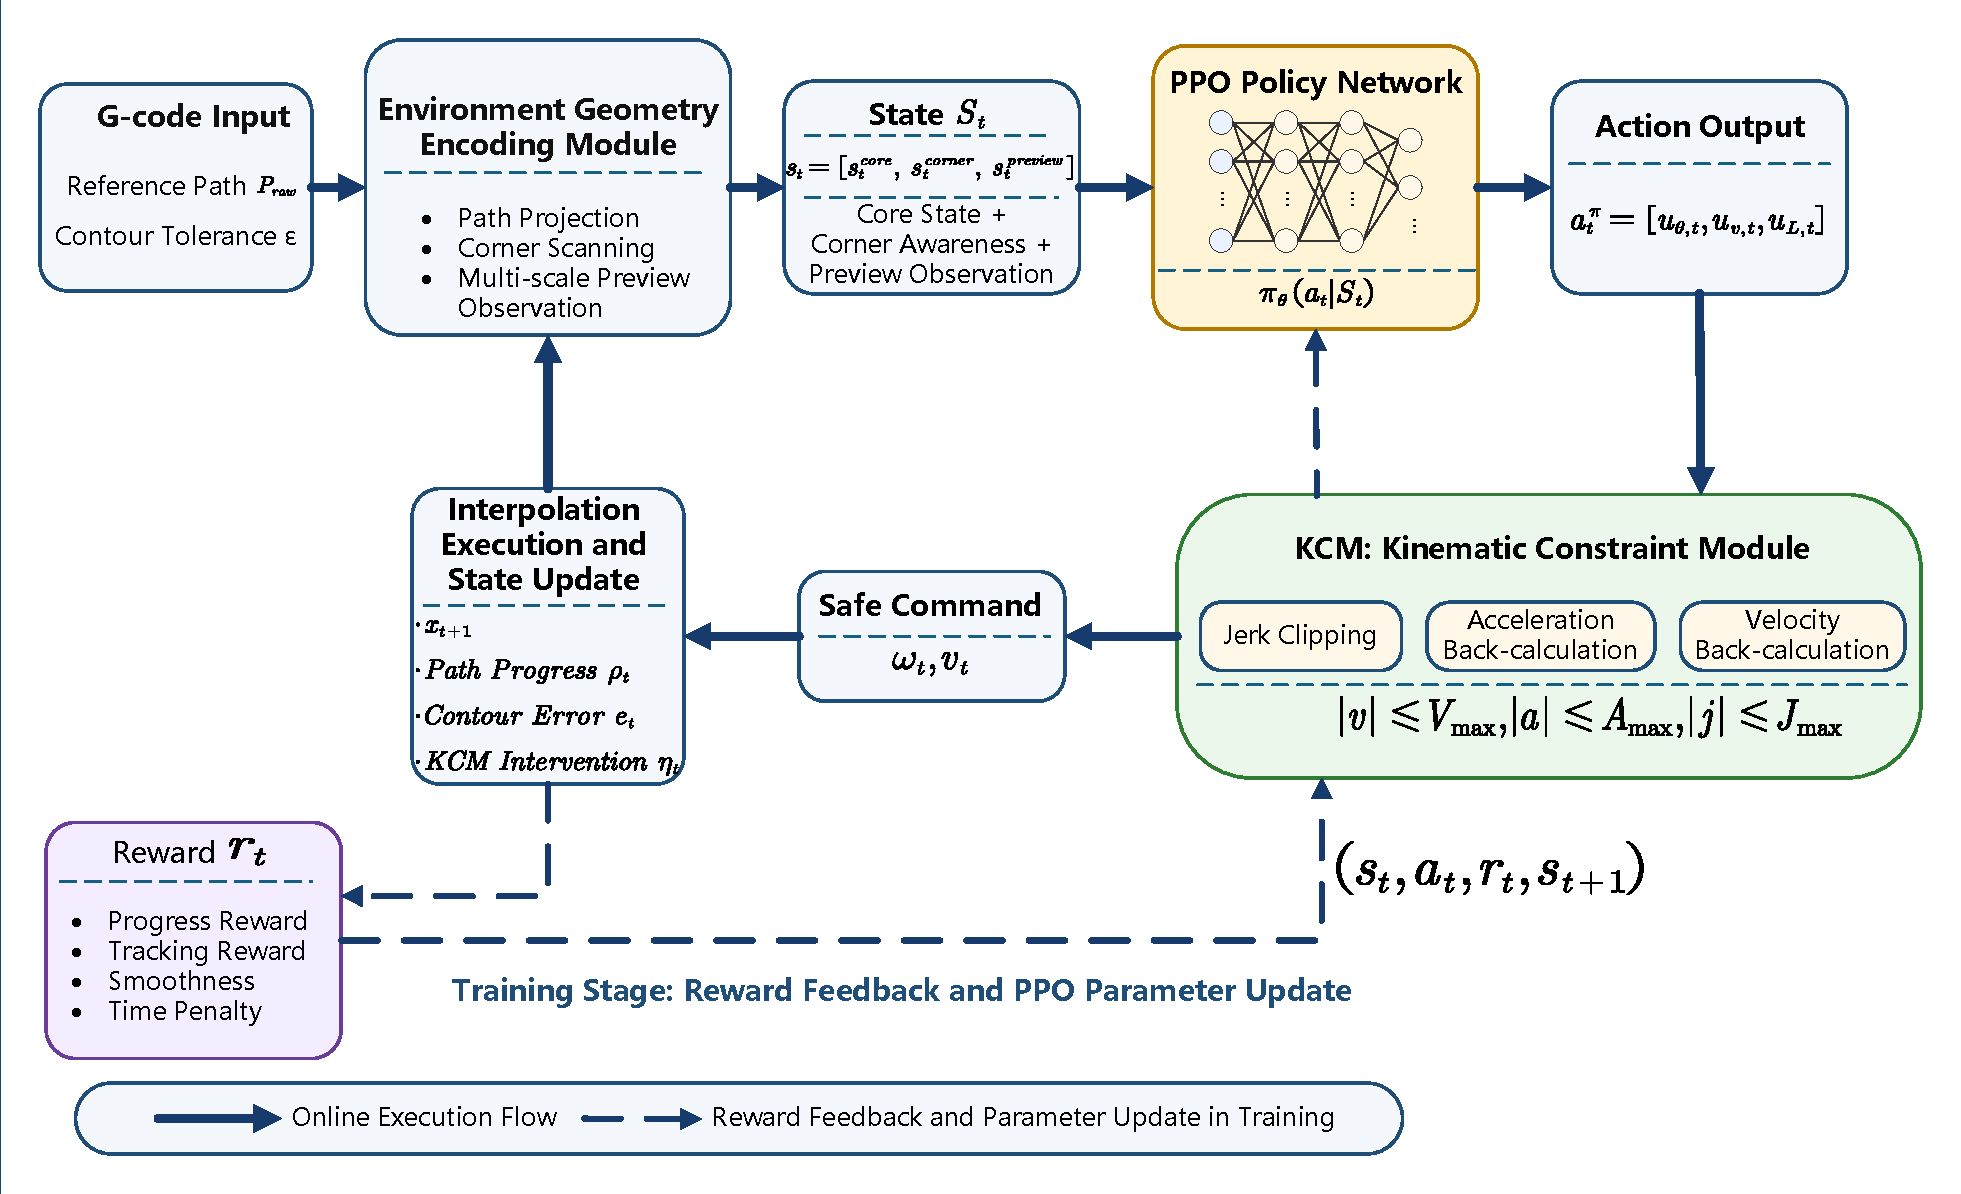
\includegraphics[width=0.9\linewidth]{fig3.pdf}
    \caption{本文方法的总体闭环框架。}
    \label{fig:framework}
\end{figure}

\subsection{结构化状态表示：核心状态、拐角感知与前瞻观测}
本文采用一种分层的结构化状态表示：
\begin{equation}
s_t=[s_t^{core},\ s_t^{corner},\ s_t^{preview}].
\end{equation}
其中 $s_t^{core}$ 描述当前时刻的局部跟踪与运动学状态，$s_t^{corner}$ 描述当前路径段与下一拐角之间的关系，$s_t^{preview}$ 描述前方若干距离处的几何变化趋势。

\paragraph{(1) 核心状态 $s_t^{core}$} 核心状态采用8维构造：
\begin{equation}
s_t^{core}=[\bar e_t,\ \bar e_{n,t},\ \bar\tau_t,\ \bar v_t,\ \bar a_t,\ \bar\omega_t,\ \rho_t,\ \bar d_{c,t}],
\end{equation}
其中 $\bar e_t$ 为归一化轮廓误差，$\bar e_{n,t}$ 为带符号法向误差，$\bar\tau_t$ 为当前航向与局部切向方向之间的归一化夹角误差，$\bar v_t$、$\bar a_t$、$\bar\omega_t$ 分别为归一化线速度、线加速度和角速度，$\rho_t\in[0,1]$ 为路径整体进度，$\bar d_{c,t}$ 为到下一拐角距离的归一化量。

\paragraph{(2) 拐角感知状态 $s_t^{corner}$} 拐角感知状态构造为4维特征：
\begin{equation}
s_t^{corner}=[\bar\phi_t,\ \sigma_t,\ m_t,\ \sigma_t\bar e_{n,t}],
\end{equation}
其中 $\bar\phi_t$ 为下一拐角转角的归一化值，$\sigma_t\in\{-1,0,1\}$ 表示拐角转向符号，$m_t\in\{0,1\}$ 表示是否处于拐角影响区间，$\sigma_t\bar e_{n,t}$ 则给出了相对于转向内侧或外侧的带符号位置关系。

\paragraph{(3) 前瞻观测 $s_t^{preview}$} 本文沿参考路径弧长方向设置若干前瞻尺度 $\{\lambda_k\}_{k=1}^{N_L}$。记当前执行点在参考路径上的投影弧长坐标为 $\ell_t$，第 $k$ 个前瞻尺度对应的前方观测点定义为
\begin{equation}
q_t^{(k)}=P_{raw}(\ell_t+\lambda_k L_t),\qquad k=1,\dots,N_L,
\end{equation}
其中 $\lambda_k$ 为尺度系数，$L_t$ 为当前周期采用的基础前瞻距离。由此，近、中、远前瞻点均沿参考路径弧长方向确定，而不是由当前执行方向上的射线交点确定。随后在每个尺度上提取前方观测点相对于当前切向的角度变化和距离比例：
\begin{equation}
s_t^{preview}=\big[\Delta \theta_t^{(1)},\ \bar d_t^{(1)},\ \dots,\ \Delta \theta_t^{(N_L)},\ \bar d_t^{(N_L)}\big].
\end{equation}
其中 $\Delta \theta_t^{(k)}$ 表征第 $k$ 个前瞻尺度上的方向变化趋势，$\bar d_t^{(k)}$ 表征当前位置到该前瞻点的归一化距离。当前实现中，主配置采用3个前瞻尺度，因此总状态维数为 $8+4+2\times 3=18$。

\subsection{动作空间与运动学约束模块}
策略网络在每个周期输出归一化动作
\begin{equation}
 a_t^{\pi}=[u_{\theta,t},u_{v,t},u_{L,t}],
\end{equation}
其中 $u_{\theta,t}\in[-1,1]$ 表示转向控制的归一化动作分量，$u_{v,t}\in[0,1]$ 表示进给控制的归一化动作分量，$u_{L,t}\in[0,1]$ 表示前瞻距离调节分量。设前瞻距离允许范围为 $[L_{\min},L_{\max}]$，则其物理量映射为
\begin{equation}
L_t=L_{\min}+u_{L,t}(L_{\max}-L_{\min}).
\end{equation}
策略输出首先被映射为物理空间中的约束前运动控制量：
\begin{equation}
\omega_t^{pre}=u_{\theta,t}\Omega_{\max},\qquad v_t^{pre}=u_{v,t}V_{\max}.
\end{equation}
前瞻距离 $L_t$ 直接参与局部参考方向与前瞻几何的计算。随后，KCM 根据上一时刻运动学状态对 $(\omega_t^{pre},v_t^{pre})$ 进行约束投影。以线速度通道为例，设上一周期的线速度和线加速度分别为 $v_{t-1}$ 与 $a_{t-1}$，则有
\begin{equation}
 a_t^{pre}=\frac{v_t^{pre}-v_{t-1}}{\Delta t},
\end{equation}
\begin{equation}
 j_t^{pre}=\frac{a_t^{pre}-a_{t-1}}{\Delta t}.
\end{equation}
KCM 首先对约束前捷度进行裁剪：
\begin{equation}
 j_t=\mathrm{clip}(j_t^{pre},-J_{\max},J_{\max}),
\end{equation}
再由此反算本周期可实现的加速度与速度：
\begin{equation}
 a_t=\mathrm{clip}(a_{t-1}+j_t\Delta t,-A_{\max},A_{\max}),
\end{equation}
\begin{equation}
 v_t=\mathrm{clip}\left(v_{t-1}+a_{t-1}\Delta t+\frac{1}{2}j_t\Delta t^2,0,V_{\max}\right).
\end{equation}
角速度通道采用完全相同的约束流程。得到的 $(\omega_t,v_t)$ 作为环境执行控制量。

本文还定义 KCM 干预度：
\begin{equation}
\eta_t=\frac{|v_t-v_t^{pre}|}{V_{\max}}+\frac{|\omega_t-\omega_t^{pre}|}{\Omega_{\max}}.
\end{equation}
该量不参与主优化目标，用于结果分析中的辅助指标。

\subsection{拐角感知奖励设计}
即时奖励写为
\begin{equation}
 r_t=r_t^{prog}+r_t^{track}+r_t^{dir}+r_t^{smooth}+r_t^{time}+r_t^{aux}.
\label{eq:reward_total}
\end{equation}

\paragraph{(1) 进度奖励} 进度奖励定义为
\begin{equation}
 r_t^{prog}=w_p\max(0,\rho_t-\rho_{t-1}),
\end{equation}
其中 $\rho_t$ 为整体路径进度。

\paragraph{(2) 轮廓误差项} 轮廓误差项定义为
\begin{equation}
\phi_e(e_t)=
\begin{cases}
0, & |e_{n,t}|\leq \delta_t,\\[4pt]
\left(\dfrac{|e_{n,t}|-\delta_t}{\varepsilon/2}\right)^2, & |e_{n,t}|>\delta_t,
\end{cases}
\end{equation}
并定义
\begin{equation}
 r_t^{track}=-w_e(c_t)\,\phi_e(e_t).
\end{equation}
其中 $\delta_t$ 为容许带内的松弛边界，$c_t\in[0,1]$ 为拐角显著性。

\paragraph{(3) 方向一致性项} 方向一致性项定义为
\begin{equation}
 r_t^{dir}=-w_{\tau}\,|\tau_t|,
\end{equation}
其中 $\tau_t$ 为当前航向与局部参考方向之间的夹角误差。

\paragraph{(4) 平滑性项} 平滑性项定义为
\begin{equation}
 r_t^{smooth}=-w_s(c_t)\,\psi_t,
\end{equation}
其中 $\psi_t$ 可取线捷度、角加速度或角捷度的归一化量；$w_s(c_t)$ 采用随拐角显著性动态变化的权重。一个常用实现为
\begin{equation}
 w_s(c_t)=w_s^0 c_t^{\gamma}, \qquad \gamma>1,
\end{equation}
其中 $w_s(c_t)$ 随 $c_t$ 增大而增大。

\paragraph{(5) 时间与辅助项} 时间项采用固定惩罚 $r_t^{time}=-w_t$。

\section{实验设计与结果}
\label{sec:experiments}

本节通过实验验证所提方法在不同几何路径下的受约束运动规划能力。实验围绕三项内容展开：路径任务完成情况、允差带内轨迹行为以及执行侧运动学约束满足情况。正文实验包括本文方法与 NNC 方法的主对照实验，以及围绕前瞻距离、KCM、前瞻观测和奖励结构的消融实验。

\subsection{实验设置}

实验在基于 Python 与 PyTorch 搭建的数控运动规划仿真环境中完成，选取正方形、圆形与蝴蝶形三条代表性路径作为测试案例。圆形路径用于考察连续转向条件下的速度保持能力，正方形路径用于考察尖角段的减速、转向与重加速能力，蝴蝶形路径用于考察长短线段与曲率变化混合条件下的轨迹规划能力。

主对照实验比较两类学习型控制方法：
\begin{enumerate}[leftmargin=2em]
    \item 本文方法：采用结构化状态表示、可学习前瞻距离、KCM 约束执行与拐角感知奖励；
    \item NNC 方法：参照 Li 等\cite{Li2020}所代表的直接神经控制思路，采用固定前瞻特征与直接神经控制结构，策略输出直接进入环境执行。
\end{enumerate}

消融实验在本文方法基础上分别移除关键模块，用于分析各组成部分对轨迹行为和动态可执行性的影响。消融配置包括：
\begin{enumerate}[leftmargin=2em]
    \item 固定前瞻：采用固定前瞻长度替代可学习前瞻距离；
    \item 无 KCM：移除执行层运动学约束投影，策略输出直接进入环境执行；
    \item 无前瞻观测：移除多尺度前瞻观测状态，保留其余模块；
    \item 无直线/拐角双奖励：移除直线区与拐角区的差异化奖励调度，仅保留统一跟踪奖励。
\end{enumerate}

评价指标包括完成率、最终进度、最大轮廓误差、线捷度最大相对超限、平均用时以及 KCM 平均干预度。其中，完成率和最终进度反映进给能力，最大轮廓误差反映允差带利用情况，线捷度最大相对超限反映动态约束满足情况，平均用时反映整体执行效率，KCM 干预度反映策略输出与运动学边界之间的匹配程度。

\subsection{主结果}

本小节给出本文方法与 NNC 方法在三条代表性路径上的对比结果。表~\ref{tab:main_results}汇总了完成率、最终进度、最大轮廓误差、线捷度最大相对超限和平均用时等指标。

\IfFileExists{generated/main_results_table.tex}{
    \begin{table}[H]
\centering
\caption{本文最终方法与基线策略在代表性路径 best rollout 上的对比结果。}
\label{tab:main_results}
\resizebox{0.92\textwidth}{!}{
\begin{tabular}{llcc}
\toprule
\textbf{路径} & \textbf{指标} & \textbf{本文最终方法} & \textbf{NNC 基线}\\
\midrule
\multirow{5}{*}{square} & 终止状态 & success & success\\
& 最终进度 & 1.000 & 1.000\\
& 最大轮廓误差 & 0.834 & 0.676\\
& 线捷度最大相对超限 & 0.000 & 3199.000\\
& 终止时间 (s) & 12.192 & 8.672\\
\midrule
\multirow{5}{*}{circle} & 终止状态 & success & max\_steps\\
& 最终进度 & 1.000 & 0.990\\
& 最大轮廓误差 & 0.096 & 6.259\\
& 线捷度最大相对超限 & 0.000 & 3199.000\\
& 终止时间 (s) & 9.117 & 60.000\\
\midrule
\multirow{5}{*}{butterfly} & 终止状态 & success & success\\
& 最终进度 & 1.000 & 1.000\\
& 最大轮廓误差 & 0.745 & 0.207\\
& 线捷度最大相对超限 & 0.000 & 3199.000\\
& 终止时间 (s) & 10.480 & 5.807\\
\bottomrule
\end{tabular}
}
\end{table}

}{
    \begin{table}[H]
    \centering
    \caption{本文最终方法与基线策略在代表性路径上的对比结果。}
    \label{tab:main_results}
    \begin{tabular}{llcc}
    \toprule
    \textbf{路径} & \textbf{指标} & \textbf{本文最终方法} & \textbf{NNC方法}\\
    \midrule
    \multirow{4}{*}{square} & 完成率 & 待填 & 待填\\
    & 最终进度 & 待填 & 待填\\
    & 最大轮廓误差 & 待填 & 待填\\
    & 线捷度超限幅度 & 待填 & 待填\\
    \midrule
    \multirow{4}{*}{circle} & 完成率 & 待填 & 待填\\
    & 最终进度 & 待填 & 待填\\
    & 最大轮廓误差 & 待填 & 待填\\
    & 线捷度超限幅度 & 待填 & 待填\\
    \midrule
    \multirow{4}{*}{butterfly} & 完成率 & 待填 & 待填\\
    & 最终进度 & 待填 & 待填\\
    & 最大轮廓误差 & 待填 & 待填\\
    & 线捷度超限幅度 & 待填 & 待填\\
    \bottomrule
    \end{tabular}
    \end{table}
}

表~\ref{tab:main_results}显示，两类学习型方法均能够在代表性路径上推进任务。本文方法在捷度最大相对超限指标上满足了约束，说明 KCM 能够将约束前运动控制量转换为满足速度、加速度与捷度边界的执行控制量。NNC 方法体现出直接神经控制的进给能力，但是出现了捷度超限的情况。

图~\ref{fig:qualitative_results}给出了三条路径上的轨迹对比。

\IfFileExists{figures/generated/qualitative_results.pdf}{
    \begin{figure}[H]
        \centering
        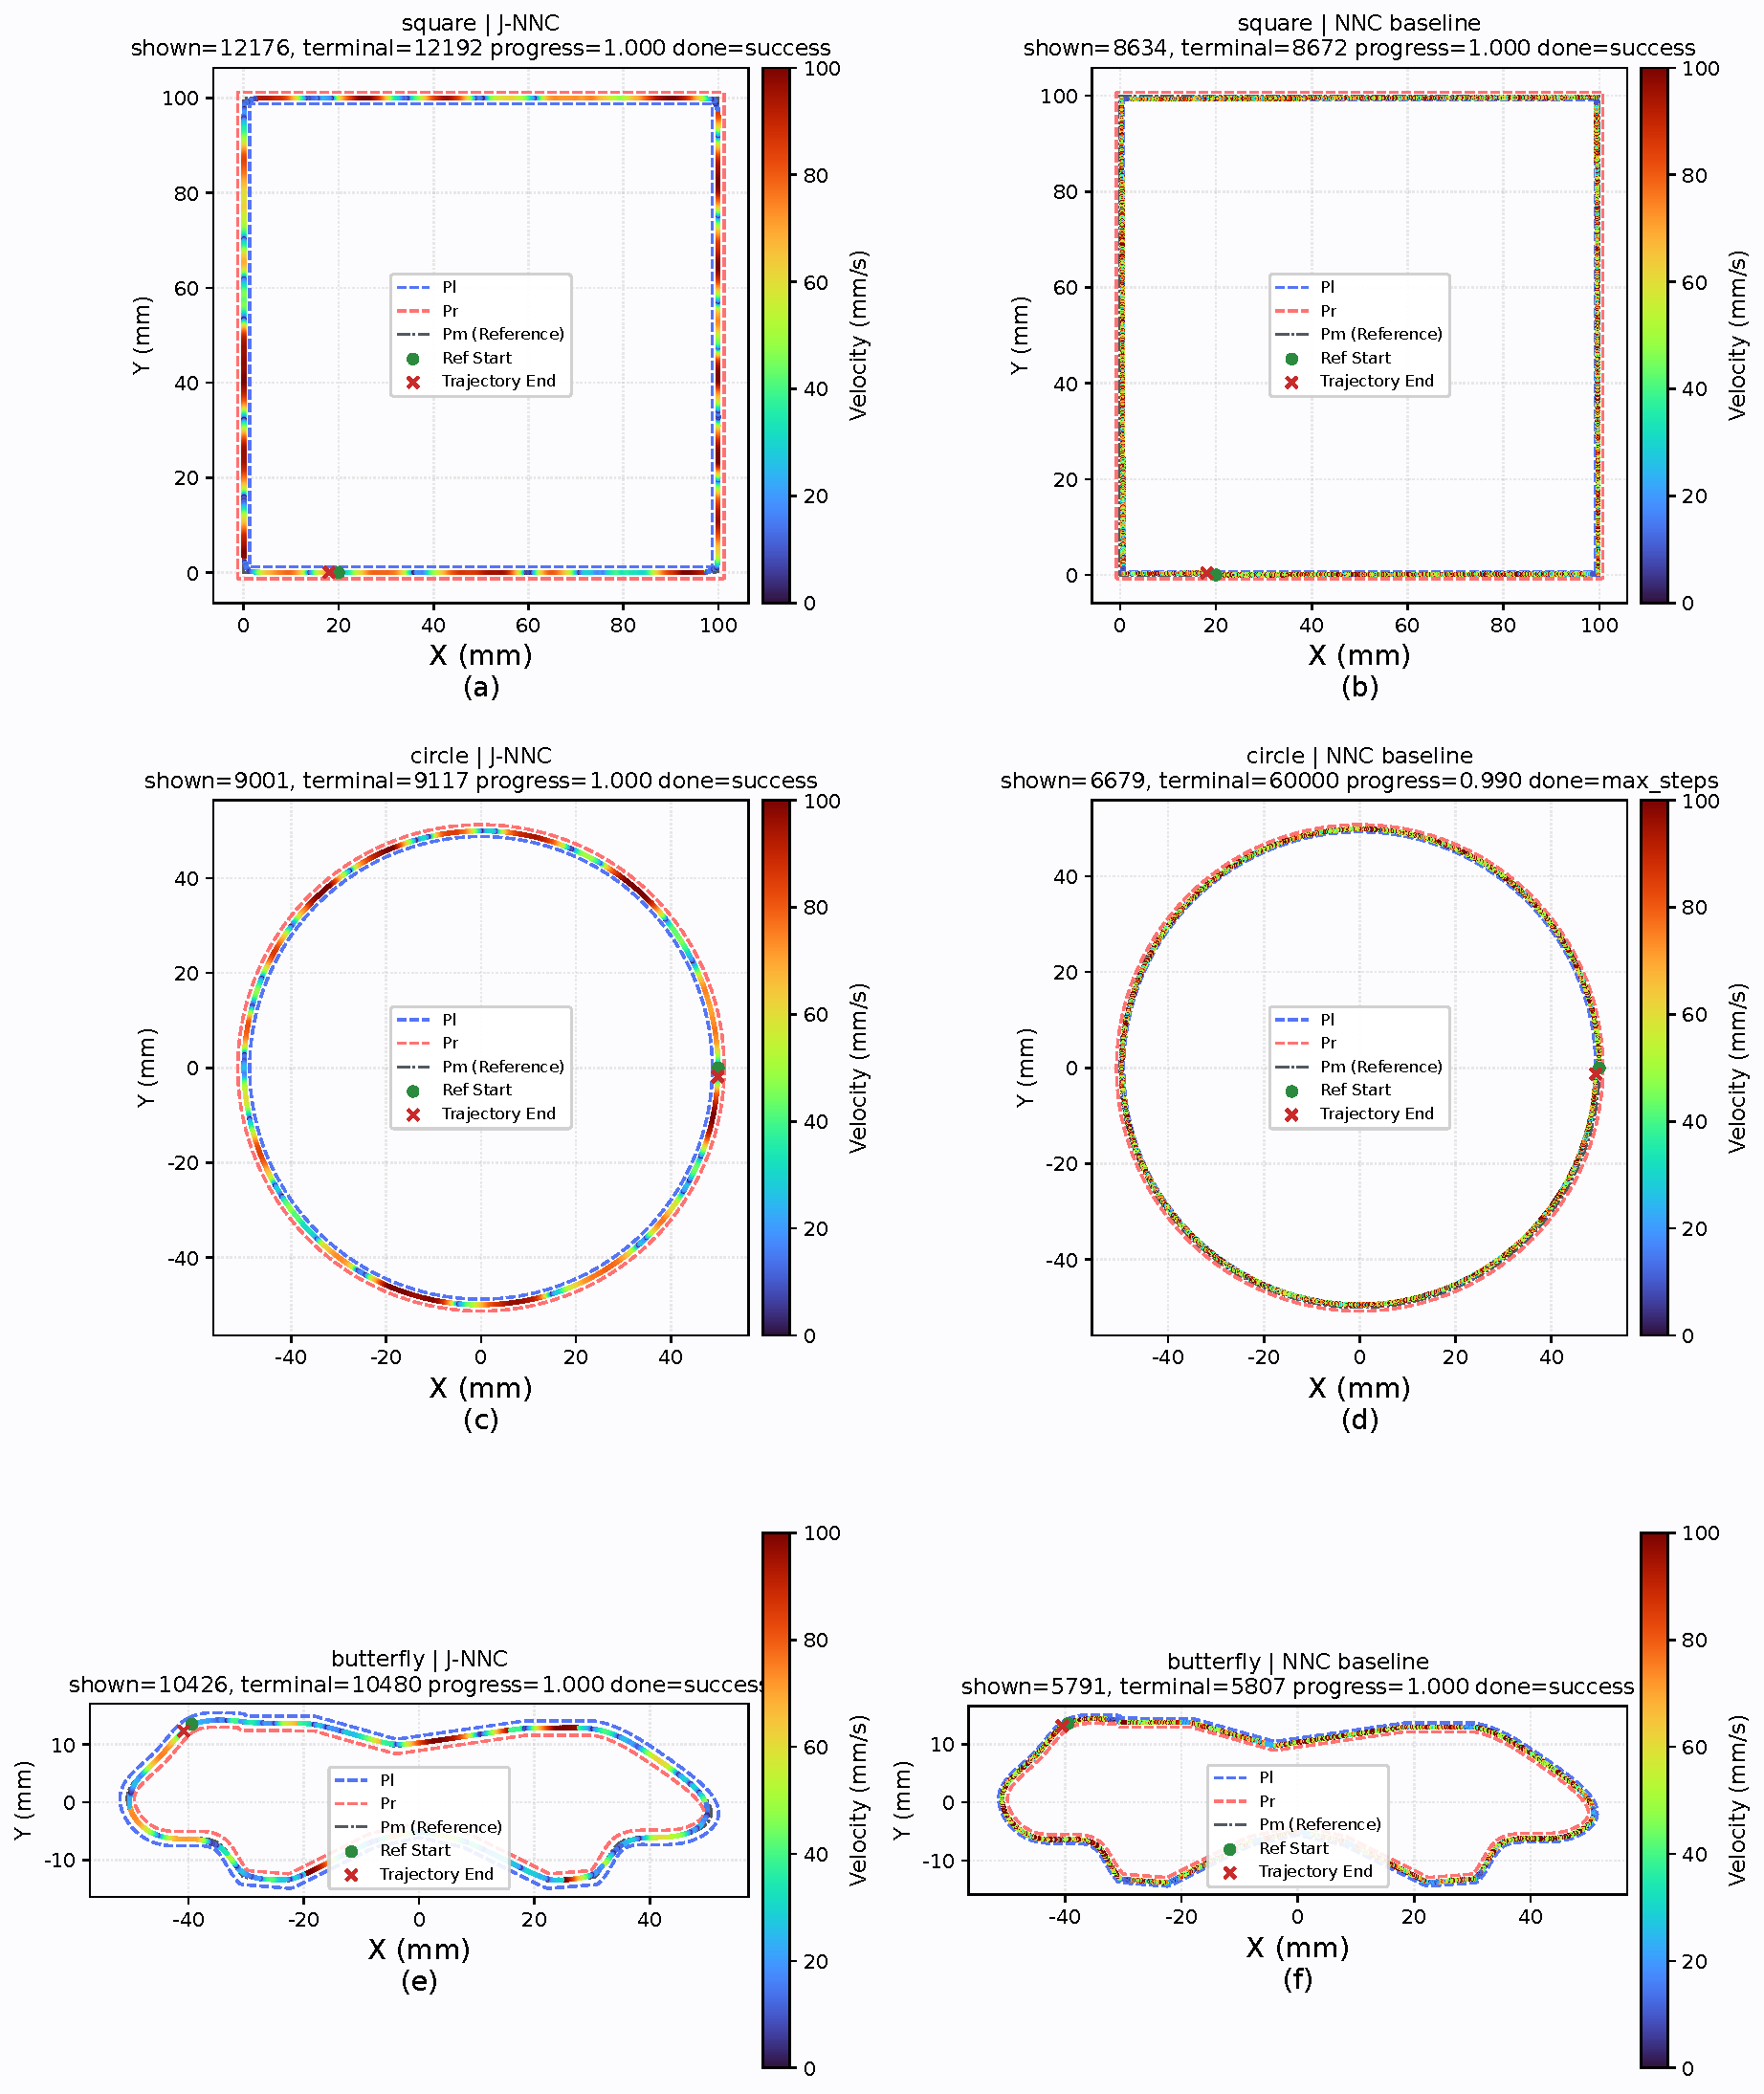
\includegraphics[width=0.96\linewidth]{figures/generated/qualitative_results.pdf}
        \caption{主方法与基线方法在代表性路径场景下的轨迹对比。}
        \label{fig:qualitative_results}
    \end{figure}
}{
    \begin{figure}[H]
        \centering
        \fbox{\parbox{0.9\linewidth}{\centering \vspace{2.8cm} 轨迹对比占位图：本文方法与基线方法在典型路径上的轨迹叠加、速度着色或局部放大图 \vspace{2.8cm}}}
        \caption{主方法与基线方法在典型路径场景下的轨迹对比。}
        \label{fig:qualitative_results}
    \end{figure}
}

圆形路径曲率连续，主要反映连续转向过程中的速度保持能力。正方形路径包含典型尖角，主要反映拐角进入、过弯和离开阶段的局部轨迹行为。蝴蝶形路径包含多尺度曲率变化，主要反映策略在复合几何条件下的推进能力。结合表~\ref{tab:main_results}可见，本文方法在不同路径上均形成有效轨迹，并通过执行层约束保持动态可执行性。

正方形路径的拐角区域对比见图~\ref{fig:square_corner_zoom}。

\IfFileExists{figures/generated/square_corner_zoom.pdf}{
    \begin{figure}[H]
        \centering
        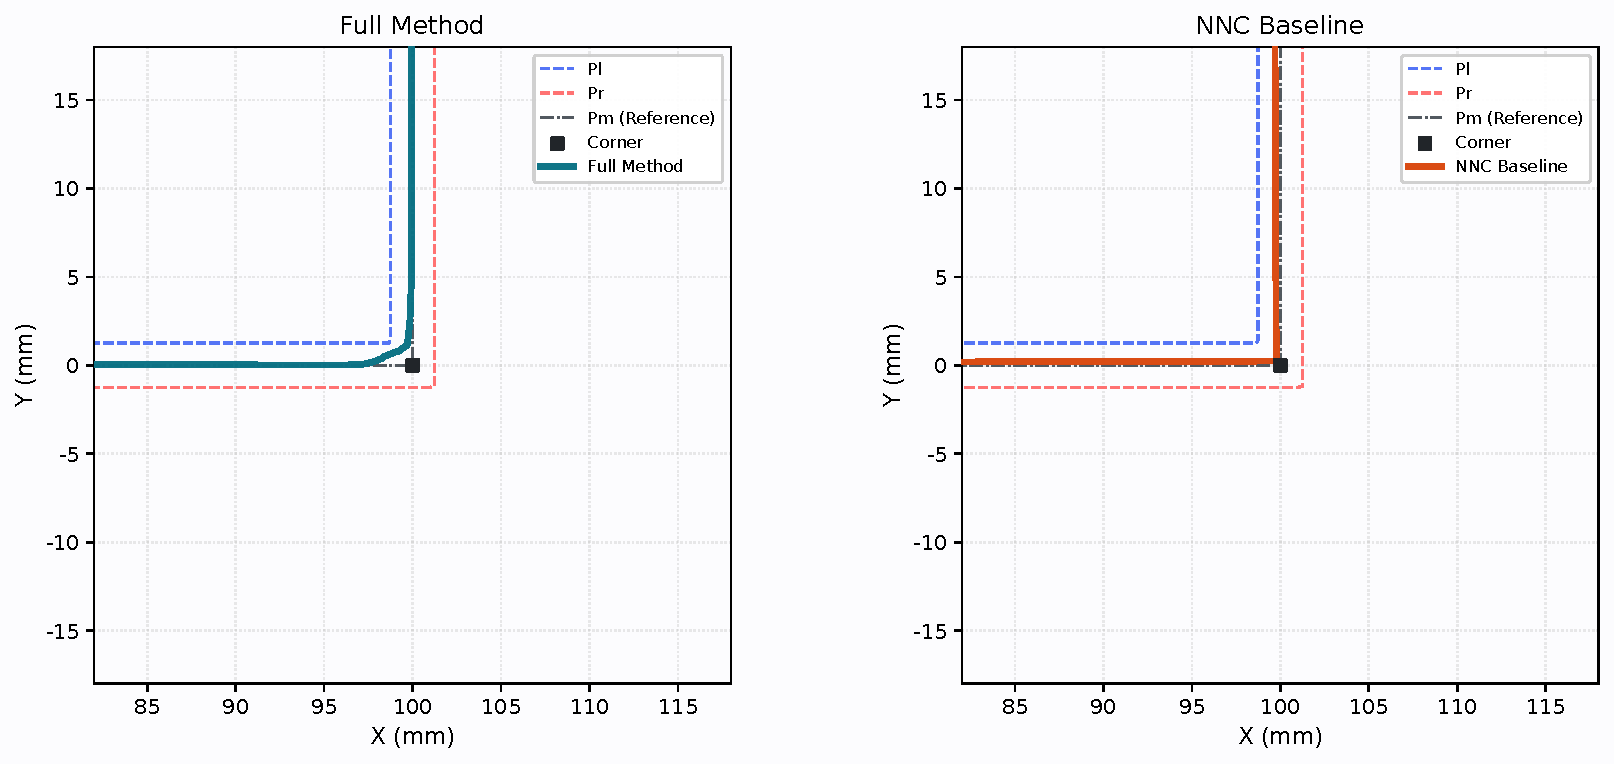
\includegraphics[width=0.92\linewidth]{figures/generated/square_corner_zoom.pdf}
        \caption{主方法与 NNC 方法在正方形路径拐角区域的局部放大轨迹对比。}
        \label{fig:square_corner_zoom}
    \end{figure}
}{
    \begin{figure}[H]
        \centering
        \fbox{\parbox{0.9\linewidth}{\centering \vspace{2.8cm} 正方形拐角局部放大占位图：主方法与基线在同一角点附近的局部轨迹高清对比 \vspace{2.8cm}}}
        \caption{主方法与 NNC 方法在正方形路径拐角区域的局部放大轨迹对比。}
        \label{fig:square_corner_zoom}
    \end{figure}
}

本文方法在角点附近利用允差带形成连续过渡轨迹，在拐角区域利用不同的奖励机制实现了拐角平滑。NNC 方法的轨迹更贴近原始折线路径，拐角点附近的方向变化更加剧烈。该结果与表~\ref{tab:main_results}中的捷度指标对应，说明本方法能够通过KCM模块和更丰富的奖励机制得到拐角平滑且满足运动学约束的轨迹。

本文方法在代表性轨迹上的轮廓误差、线捷度与 KCM 干预度如图~\ref{fig:kcm_analysis}所示。

\IfFileExists{figures/generated/kcm_analysis.pdf}{
    \begin{figure}[H]
        \centering
        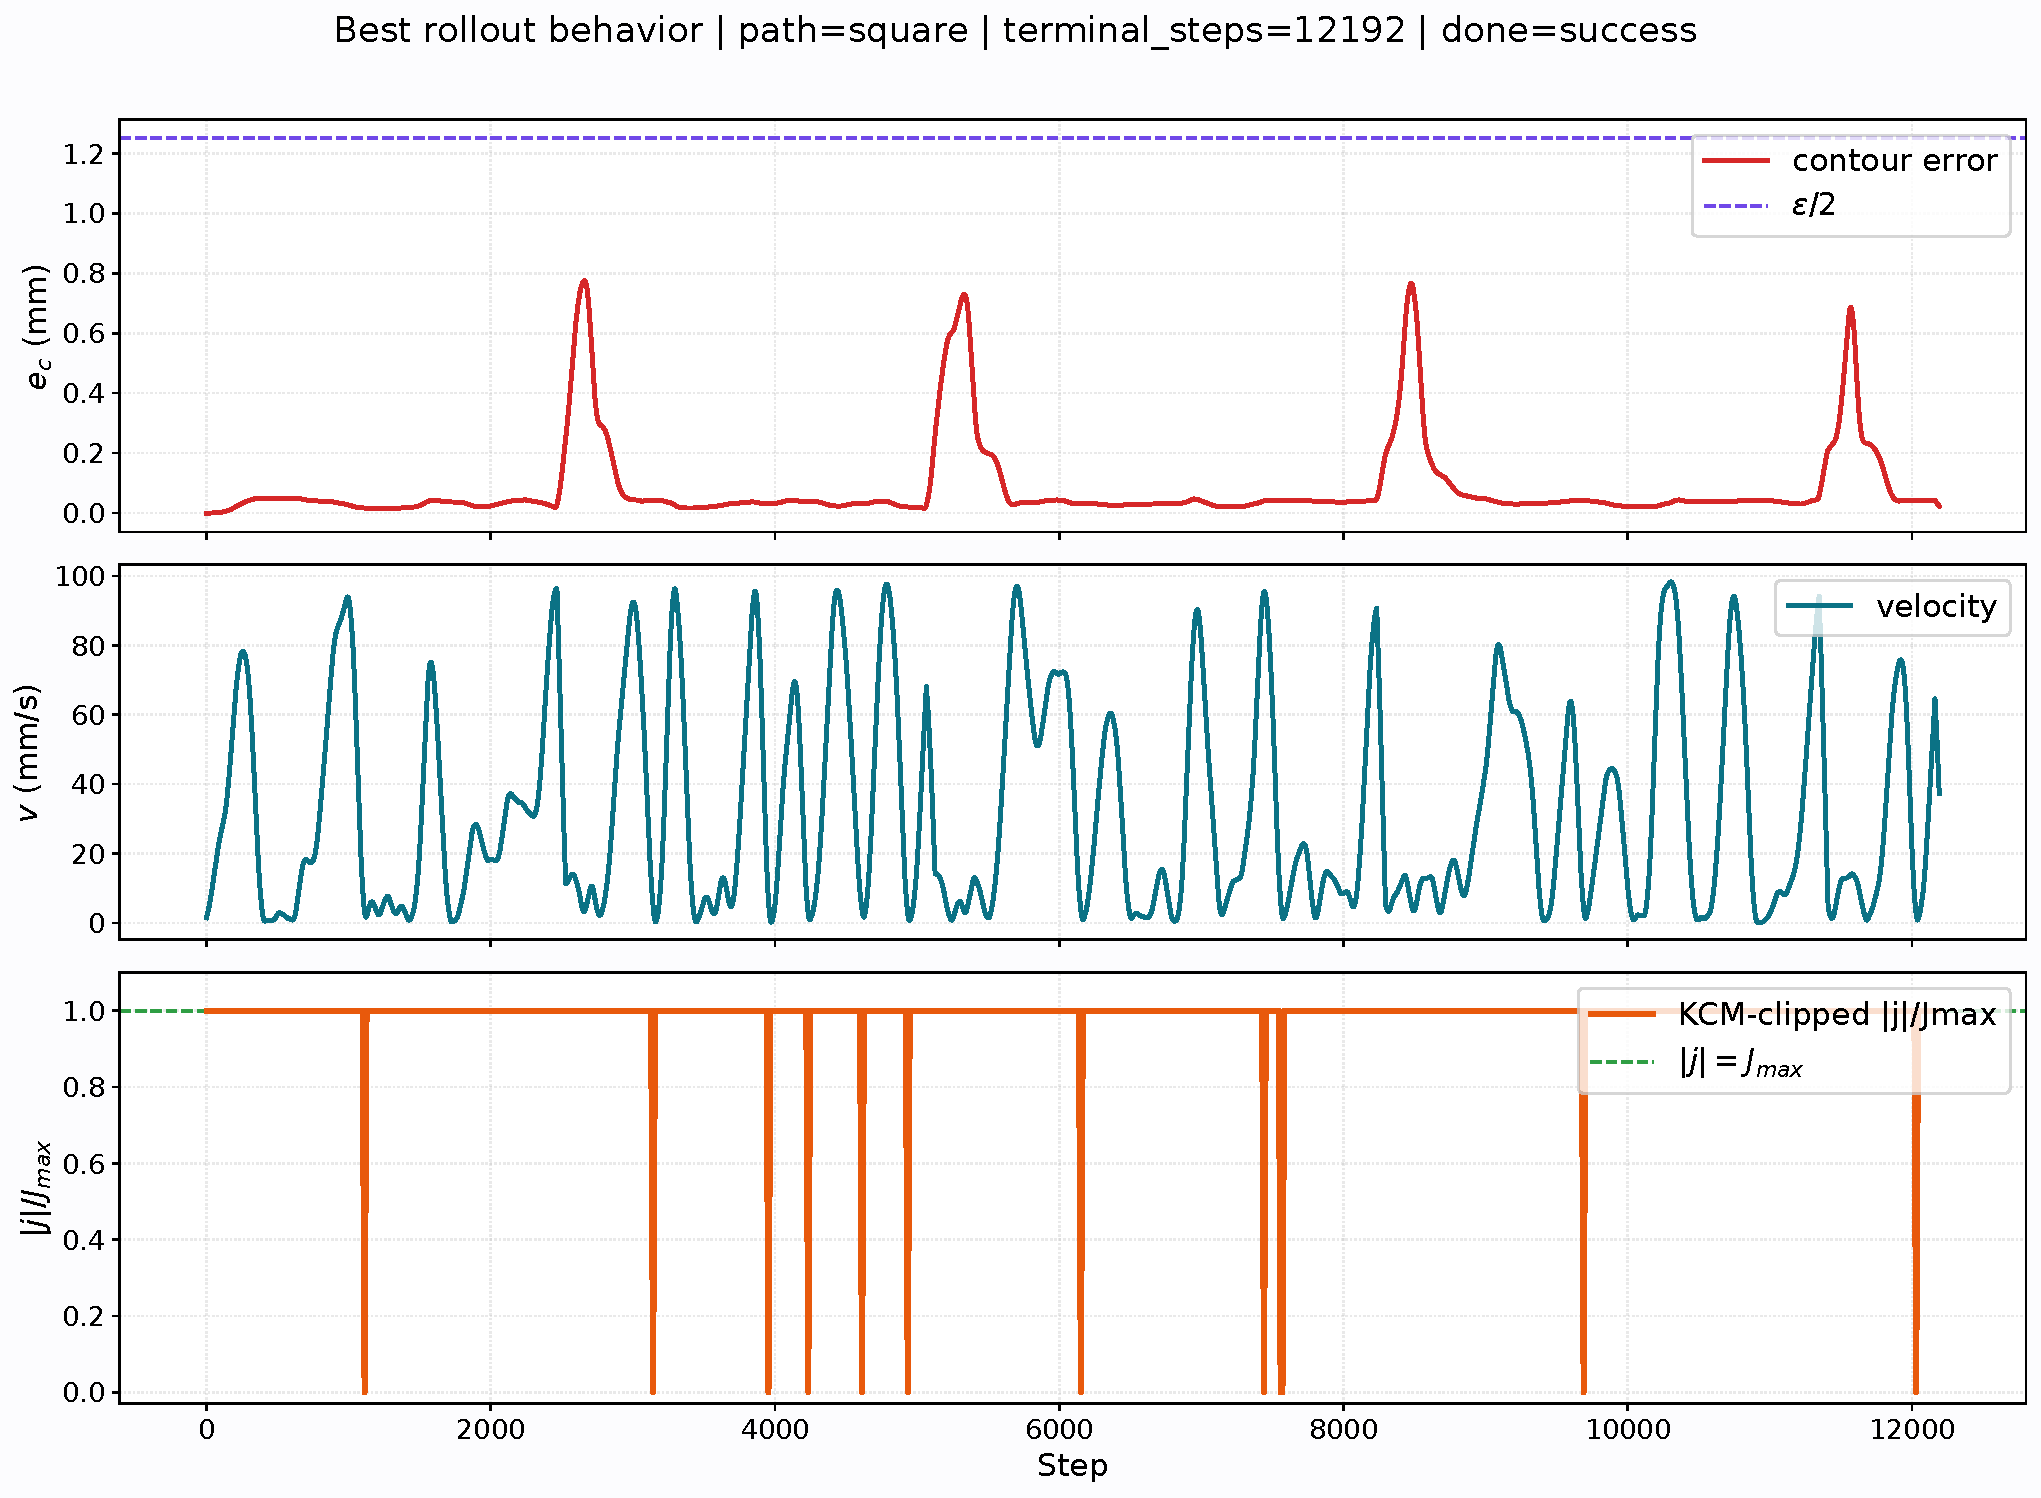
\includegraphics[width=0.96\linewidth]{figures/generated/kcm_analysis.pdf}
        \caption{本文最终方法在选定代表性轨迹上的轮廓误差、线捷度与 KCM 干预度时序图。}
        \label{fig:kcm_analysis}
    \end{figure}
}{
    \begin{figure}[H]
        \centering
        \fbox{\parbox{0.9\linewidth}{\centering \vspace{2.8cm} 行为解释占位图：前瞻距离、KCM干预度、误差和速度在拐角区的时序对齐图 \vspace{2.8cm}}}
        \caption{前瞻调节、KCM干预度与拐角行为解释图。}
        \label{fig:kcm_analysis}
    \end{figure}
}

轮廓误差峰值主要分布在拐角阶段，体现了策略对允差带的局部利用。线捷度曲线保持在给定边界内，体现了 KCM 对执行控制量的约束作用。KCM 干预度在起步阶段和拐角阶段较为明显，表明约束投影主要作用于速度变化和方向变化集中的区间。

综合表~\ref{tab:main_results}与图~\ref{fig:qualitative_results}至图~\ref{fig:kcm_analysis}可以看出，本文方法在三类路径上均具备稳定的路径推进能力，并能够在允差带内形成局部平滑轨迹。对于正方形尖角和蝴蝶形混合曲率区域，轨迹的适当偏移得到了更平滑的拐角过渡以及严格满足运动学约束。NNC 方法体现出直接神经控制进给的能力，暴露出奖励机制简单以及没有显示约束处理导致的可执行性问题。

\subsection{消融实验结果}

本小节给出可学习前瞻距离、KCM、前瞻观测以及直线/拐角双奖励等模块的消融结果。表~\ref{tab:ablation}汇总了不同配置下的完成路径数、均值末进度、全局最大轮廓误差、平均用时和 KCM 干预度。

\IfFileExists{generated/ablation_table.tex}{
    \begin{table}[H]
\centering
\caption{Path-level results of the structured ablation study.}
\label{tab:ablation}
\begingroup
\small
\setlength{\tabcolsep}{3pt}
\renewcommand{\arraystretch}{1.16}
\resizebox{0.98\textwidth}{!}{%
\begin{tabular}{>{\raggedright\arraybackslash}p{0.23\textwidth}lccccc}
\toprule
\textbf{Configuration} & \textbf{Path} & \textbf{Outcome} & \textbf{Final progress} & \begin{tabular}[c]{@{}c@{}}\textbf{Peak contour}\\\textbf{error [mm]}\end{tabular} & \begin{tabular}[c]{@{}c@{}}\textbf{Peak jerk-limit}\\\textbf{exceedance}\end{tabular} & \textbf{Elapsed time [s]}\\
\midrule
\multirow{3}{0.23\textwidth}{J-NNC} & square & success & 1.000 & 0.834 & 0.000 & 12.192\\
& circle & success & 1.000 & 0.096 & 0.000 & 9.117\\
& butterfly & success & 1.000 & 0.745 & 0.000 & 10.480\\
\addlinespace[0.35em]
\multirow{3}{0.23\textwidth}{Fixed Adaptive Preview} & square & success & 1.000 & 0.699 & 0.000 & 8.680\\
& circle & success & 1.000 & 0.046 & 0.000 & 4.804\\
& butterfly & success & 1.000 & 0.638 & 0.000 & 5.049\\
\addlinespace[0.35em]
\multirow{3}{0.23\textwidth}{Without KCM} & square & success & 1.000 & 0.722 & 3199.000 & 10.301\\
& circle & success & 1.000 & 0.061 & 3199.000 & 5.926\\
& butterfly & success & 1.000 & 0.707 & 3199.000 & 7.446\\
\addlinespace[0.35em]
\multirow{3}{0.23\textwidth}{Without Adaptive Preview observation} & square & success & 1.000 & 0.805 & 0.000 & 8.151\\
& circle & success & 1.000 & 0.077 & 0.000 & 4.573\\
& butterfly & success & 1.000 & 0.820 & 0.000 & 6.044\\
\addlinespace[0.35em]
\multirow{3}{0.23\textwidth}{Without straight-line/corner dual rewards} & square & success & 1.000 & 0.824 & 0.000 & 15.132\\
& circle & success & 1.000 & 0.030 & 0.000 & 10.388\\
& butterfly & success & 1.000 & 0.918 & 0.000 & 9.623\\
\bottomrule
\end{tabular}
}
\endgroup
\end{table}

}{
    \begin{table}[H]
    \centering
    \caption{结构化消融结果汇总。}
    \label{tab:ablation}
    \begin{tabular}{lccccc}
    \toprule
    \textbf{模型配置} & \textbf{完成路径数} & \textbf{均值末进度} & \textbf{全局最大轮廓误差} & \textbf{平均用时 (s)} & \textbf{平均KCM干预度}\\
    \midrule
    本文最终方法 & 待填 & 待填 & 待填 & 待填 & 待填\\
    固定前瞻 & 待填 & 待填 & 待填 & 待填 & 待填\\
    无KCM & 待填 & 待填 & 待填 & 待填 & 待填\\
    无前瞻观测 & 待填 & 待填 & 待填 & 待填 & 待填\\
    无直线/拐角双奖励 & 待填 & 待填 & 待填 & 待填 & 待填\\
    \bottomrule
    \end{tabular}
    \end{table}
}

表~\ref{tab:ablation}显示，KCM、前瞻信息和奖励结构分别影响动态可执行性、几何感知能力和跨路径稳定性。固定前瞻配置反映了前瞻距离在线调节的影响，无前瞻观测配置反映了多尺度几何信息的影响，无直线/拐角双奖励配置反映了阶段化奖励调度的影响，无 KCM 配置用于分析执行层约束投影的作用。

本文最终方法与无 KCM 配置在相同代表性路径上的线捷度对比如图~\ref{fig:jerk_constraint_comparison}所示。

\IfFileExists{figures/generated/jerk_constraint_comparison.pdf}{
    \begin{figure}[H]
        \centering
        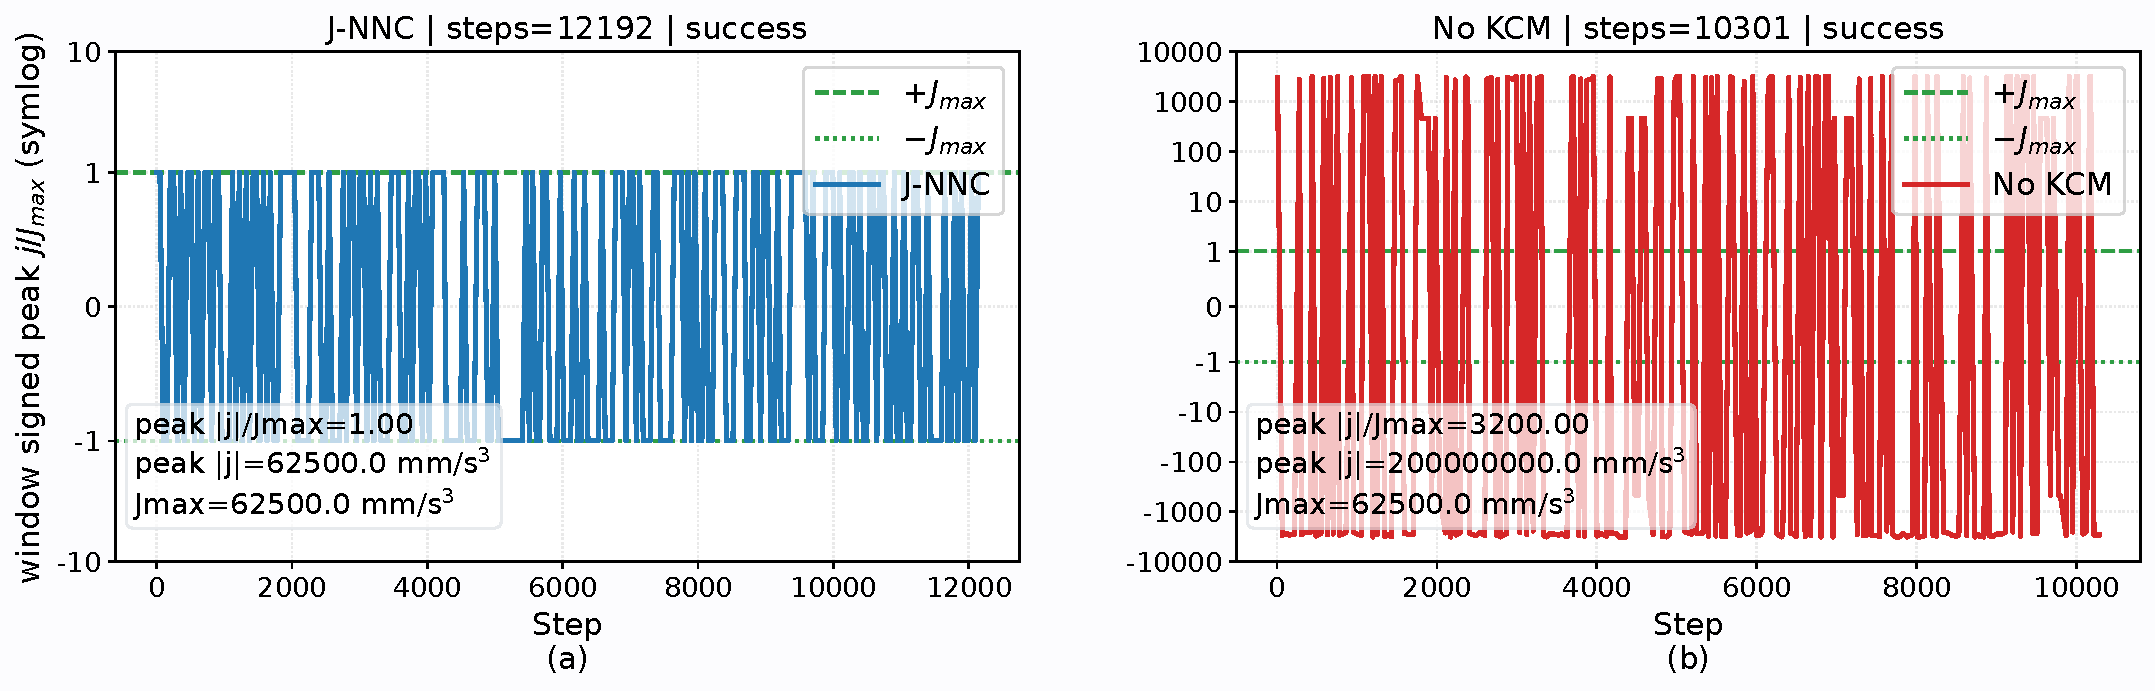
\includegraphics[width=0.96\linewidth]{figures/generated/jerk_constraint_comparison.pdf}
        \caption{本文最终方法与无 KCM 消融在相同代表性路径上的线捷度与捷度约束对比。}
        \label{fig:jerk_constraint_comparison}
    \end{figure}
}{
    \begin{figure}[H]
        \centering
        \fbox{\parbox{0.9\linewidth}{\centering \vspace{2.8cm} 捷度约束对比占位图：本文最终方法与无KCM消融在相同路径上的线捷度及其约束上界对比 \vspace{2.8cm}}}
        \caption{本文最终方法与无 KCM 消融在相同代表性路径上的线捷度与捷度约束对比。}
        \label{fig:jerk_constraint_comparison}
    \end{figure}
}

本文最终方法的捷度始终保持在 $J_{\max}$ 边界内，无 KCM 配置在训练中中出现高幅值捷度尖峰。该结果说明，KCM 对约束前运动控制量进行投影，使执行控制量满足速度、加速度与捷度边界。也说明了路径推进指标需要与运动学约束指标共同评价，以全面反映策略的受约束运动规划能力。

固定前瞻配置用于观察前瞻距离调节分量的作用。该配置保留前方几何感知结构，采用固定前瞻长度进行决策。结合表~\ref{tab:ablation}可见，固定前瞻在当前路径集合中具备较强的路径推进能力。可学习前瞻距离为策略提供了在线调节感知尺度的自由度，同时增加了动作空间维度，其效果与路径复杂度、奖励权重和 KCM 干预程度相关。

无前瞻观测配置用于观察多尺度前方几何信息的作用。该配置保留可学习前瞻距离和 KCM 约束执行，移除多尺度前瞻观测状态。结合表~\ref{tab:ablation}可见，局部状态和拐角感知能够支撑当前三条路径的基本推进。多尺度前瞻观测为策略提供更完整的前方几何趋势信息，主要作用于复杂混合路径中的提前调速和拐角预处理。

无直线/拐角双奖励配置用于观察阶段化奖励调度的作用。该配置采用统一奖励权重处理直线进给、进入拐角、过弯和离开阶段。结合表~\ref{tab:ablation}可见，移除该模块后跨路径完成稳定性下降。直线/拐角双奖励能够分别约束直线段的持续进给行为和拐角段的平滑过渡行为。

综合表~\ref{tab:ablation}与图~\ref{fig:jerk_constraint_comparison}可以看出，KCM 主要保证执行轨迹的动态可行性，直线/拐角双奖励主要保证不同几何阶段的行为稳定性，可学习前瞻距离与多尺度前瞻观测主要提供前方几何感知与在线调节能力。完整的方法通过上述模块协同实现允差带内轨迹规划、路径进给和运动学约束满足。

\section{局限性分析与未来展望}
\label{sec:conclusion}

本文方法仍有若干不足。首先，可学习前瞻距离虽然增加了在线调节自由度，但在当前实验中，其优势尚未稳定转化为更短用时或更低 KCM 干预度，说明前瞻距离分量的参数化方式仍需改进。其次，方法在不同几何路径上的表现还不完全均衡。对于连续曲率路径，策略较容易形成稳定的速度调节；对于含尖角或混合曲率变化的路径，阶段切换、终点收敛和局部过弯仍是主要难点。最后，KCM 能够保证执行控制量满足运动学约束，但较高的干预度也说明策略本体尚未充分学会贴合约束边界的控制规律。

后续工作将从三方面展开。第一，改进动作空间中前瞻距离分量的参数化方式，例如采用残差式、分段式或与拐角相位相关的前瞻参数化，以降低学习难度并减少与前瞻观测之间的冗余。第二，细化拐角阶段建模，重点处理尖角进入、过弯、离开和终点停止等局部过程，提高复杂路径下的完成率与速度衔接稳定性。第三，扩大测试路径集合，并进一步引入伺服滞后、轴向约束和实机加工条件，使仿真中的允差带利用、时间效率和捷度约束评价逐步接近实际 CNC 运动规划需求。

\appendix

\section{}

\begin{algorithm}[htbp]
\caption{KCM约束投影过程}
\label{alg:kcm}
\begin{algorithmic}[1]
\Require 策略输出 $a_t^{\pi}=[u_{\theta,t},u_{v,t},u_{L,t}]$；上一时刻运动学状态 $(v_{t-1},a_{t-1},\omega_{t-1},\alpha_{t-1})$
\Ensure 执行控制量 $(\omega_t,v_t)$ 及更新后的运动学状态
\State 将 $u_{\theta,t}$ 与 $u_{v,t}$ 映射为约束前运动控制量 $(\omega_t^{pre},v_t^{pre})$
\State 将 $u_{L,t}$ 映射为当前前瞻距离 $L_t$
\State 根据 $v_t^{pre}$ 与 $v_{t-1}$ 计算约束前线加速度 $a_t^{pre}$
\State 根据 $a_t^{pre}$ 与 $a_{t-1}$ 计算约束前线捷度 $j_t^{pre}$
\State 对 $j_t^{pre}$ 进行裁剪，得到满足上限的 $j_t$
\State 由 $j_t$ 反算线加速度 $a_t$，并执行加速度裁剪
\State 由 $(v_{t-1},a_{t-1},j_t)$ 积分得到本周期线速度 $v_t$
\State 对角速度通道采用同构流程，得到约束后的 $\omega_t$
\State 返回执行控制量 $(\omega_t,v_t)$ 及相应更新后的运动学状态
\end{algorithmic}
\end{algorithm}

\end{document}